\section{Experiments}
\label{sec:application}

We evaluate IASA in controlled experiments with known contributions
(Section~\ref{subsec:pollution_controlled}) and on four observed weeks without ground
truth (Section~\ref{subsec:observed_results}).

\subsection{Controlled Experiments}
\label{subsec:pollution_controlled}

The controlled experiments generate PM\(_{2.5}\) readings from known nonnegative
contributions with the puff model of Section~\ref{sec:problem_setup} on the
\(40\times40\) grid, so that the error of every reported quantity can be measured.  Each
run covers 72 hours, mostly with two source groups, and varies one factor at a time:
wind, sensor layout, nuisance basis, noise, operator error, lag, temporal basis or
inventory.  Unless the factor is varied, the sensors are the 32 regulatory locations,
with three downwind sensors in Experiment 10 and six random ones in the steady-wind
case of Experiment 11.  The sources are compact synthetic emitters except in
Experiments 2, 6 and 8, which use the New Delhi maps, and the winds are synthetic
except where real wind is stated
(Appendices~\ref{app:pollution_experiments}--\ref{app:additional_experiments}).  Coefficient error is
\(\|\widehat{\mathbf c}-\mathbf c\|_2/\|\mathbf c\|_2\), the group-signal error of a
reported block \(G\) is \(\|\At_G(\widehat{\mathbf c}_G-\mathbf c_G)\|_2/\|\At_G\mathbf c_G\|_2\),
and noise is Gaussian with standard deviation stated as a fraction of the largest
absolute noiseless source signal of that run.

\begin{figure*}[t]
\centering
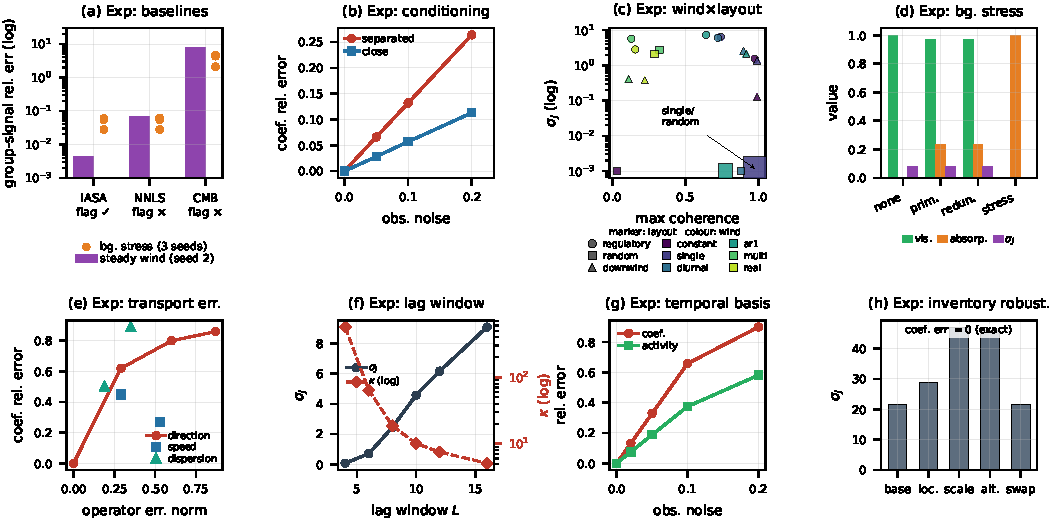
\includegraphics[width=\textwidth]{figures/fig_controlled.pdf}
\caption{Controlled experiments on the New Delhi platform.  \textbf{(a)}~Largest
relative group-signal error of IASA and two baselines that raise no identifiability
flag (plain NNLS on the projected system, a mass balance on the unprojected
response): background stress over three seeds (points) and the steady-wind case in the
seed where the plumes reach the sensors (bars).  \textbf{(b)}~Coefficient error against
noise for two sources \(4\) cells apart (\(\sigma_J=9.6\), \(\kappa=2.3\)) and \(20\)
cells apart (\(\sigma_J=3.3\), \(\kappa=8.9\)).  \textbf{(c)}~\(\sigma_J\) against maximum
coherence across wind providers (colour, with ar1 denoting AR(1) wind) and sensor
layouts (marker), where marker size increases with coefficient error and \(\sigma_J\)
below \(10^{-3}\) is drawn at \(10^{-3}\).  \textbf{(d)}~Nuisance bases none, primary
(rank 4), redundant (same span) and stress (source-like column): the stress basis drives
absorption to \(1\) and \(\sigma_J\) and the visibility ratio
\(\|\at_j\|_2/\|\mathbf a_j\|_2\) to \(0\).
\textbf{(e)}~Coefficient error against operator-error norm along the wind-direction,
wind-speed and dispersion axes.  \textbf{(f)}~\(\sigma_J\) and \(\kappa\) against the lag
window.  \textbf{(g)}~Activity error and coefficient error against noise.
\textbf{(h)}~\(\sigma_J\) across inventory versions.}
\label{fig:controlled}
\end{figure*}

\noindent\textbf{Baselines on two controlled degeneracies.}
IASA is compared over three seeds with plain NNLS on the projected system (the same
estimator without grouping and diagnostics), a transport-based mass balance (CMB: NNLS
on the unprojected response, with transport columns in place of chemical profiles) and
a nonnegative matrix factorization of the sensor-by-hour readings (PMF/NMF)
(Figure~\ref{fig:controlled}(a), Table~\ref{tab:results_baselines}).  Every method is
scored on IASA's reported blocks, errors range over those blocks, and share error is
the \(L_2\) distance between share vectors.  \emph{Source-like background} (32 regulatory
sensors, two sources with two columns each): a declared nuisance column is
proportional to one basis column of source A, whose norm falls from \(0.081\) to
\(10^{-16}\) under projection.  IASA flags it (absorption \(1\)), the two sources
have separation above \(0.9999\), and IASA's group-signal errors are
\(0.4\)--\(6.0\%\), with share errors \(0.003\)--\(0.007\).  Plain
NNLS gives group-signal errors within \(0.003\) of IASA's and raises no flag.  CMB,
without nuisance removal, has group-signal errors of \(36\)--\(463\%\) and share errors
\(0.12\)--\(0.19\).  \emph{Steady wind}
(one wind direction, six random sensors): in two seeds neither plume reaches the
sensors (column norms below \(10^{-10}\), against \(0.062\) and \(0.067\) in the third), and
IASA flags \(\sigma_J\approx0\).  In the third seed the two columns have coherence
\(0.99966\) and separation \(0.026<\tau_\theta\), so no reportable partition has two
blocks.  IASA therefore merges them, and the merged signal has error \(0.44\%\), against
\(784\%\) for CMB.
Reported separately, as plain NNLS reports them, the two sources' signals have errors of
\(3.8\%\) and \(6.9\%\).  PMF/NMF has share errors on the unprojected response of
\(1.15\)--\(1.19\) (background stress) and \(0.30\) (steady wind), and no baseline raises
a flag in either scenario.

\begin{table}[t]
\centering
\footnotesize
\setlength{\tabcolsep}{3pt}
\caption{Experiment 11: largest relative group-signal error of the reported blocks
(background stress in seeds \(0\), \(1\) and \(2\), and steady wind in seed \(2\), the only
seed with signal at the sensors).  Share errors: Table~\ref{tab:results_baselines_full}.}
\label{tab:results_baselines}
\vspace{3pt}
\begin{tabular}{llcc}
\toprule
method & flag & background stress & steady wind \\
\midrule
IASA & yes & \(0.054,\,0.028,\,0.060\) & \(0.004\) (merged) \\
plain NNLS & no & \(0.054,\,0.028,\,0.062\) & \(0.004\) \\
CMB & no & \(4.63,\,2.10,\,4.32\) & \(7.84\) \\
\bottomrule
\end{tabular}
\end{table}

\noindent\textbf{Conditioning and noise (Experiment 1).}
For two full-rank geometries, coefficient error is zero without noise and grows
linearly with it (one noise draw, scaled): \(0.066\), \(0.132\), \(0.264\) at noise
\(0.05\), \(0.10\), \(0.20\) for \(\sigma_J=3.27\), against \(0.028\), \(0.057\), \(0.113\)
for \(\sigma_J=9.60\) (Figure~\ref{fig:controlled}(b), Table~\ref{tab:results_h1}),
consistent with Proposition~\ref{prop:noise_robust}.

\noindent\textbf{Sensor layout and wind (Experiment 4).}
With the 32 regulatory locations, \(\sigma_J\ge1.53\) under all six winds, and the
maximum coherence falls from \(0.975\) under a constant wind to \(0.129\) and \(0.156\)
under multi-directional and real New Delhi wind (Figure~\ref{fig:controlled}(c),
Table~\ref{tab:results_h4}).  With eight randomly placed sensors and four of the six
winds, source B's operator column has norm \(5.2\times10^{-7}\) to \(1.7\times10^{-4}\),
against \(7.6\)--\(18.6\) with the regulatory layout, so \(\sigma_J\approx0\) and the
largest coefficient error of the sweep (\(0.573\)) is that source's poorly determined
coefficient (\(\sigma_J\approx10^{-6}\)).  The layouts also differ in sensor count.

\noindent\textbf{Nuisance absorption and missing sources (Experiments 3 and 8).}
A source-like nuisance basis drives the absorption of one column to \(1\) and
\(\sigma_J\) to \(0\) while the fitted residual is unchanged (Figure~\ref{fig:controlled}(d),
Table~\ref{tab:results_h3}), and the coefficient error falls (\(0.78\) with the
source-like basis against \(2.61\) with the rank-4 basis) because the signal has been
absorbed, so the error alone would not reveal the problem.
The adequacy test (\(\alpha=0.05\), \(1{,}000\) replicates) rejects at rate \(0.05\) under
a correct model and \(1.00\) when an omitted source has \(91\%\) of its signal outside the
span of \(A(\omega)\) and \(Q\), whereas an omitted source equal to a nonnegative
combination of the fitted columns plus nuisance columns is absorbed and rejected at rate
\(0.05\)
(Table~\ref{tab:results_missing}).  A non-rejection therefore does not show that the inventory is complete.

\noindent\textbf{Transport error (Experiment 5).}
This experiment measures the operator error of
Proposition~\ref{prop:operator_perturbation}.  Fitting with a perturbed operator
(Figure~\ref{fig:controlled}(e), Table~\ref{tab:results_h5a}), the coefficient error reaches \(0.62\) at a \(5^\circ\) error in wind
direction, \(0.86\) at \(20^\circ\) and \(0.89\) at twice the dispersion, while along the
speed axis it is not monotonic (\(0.45\) at \(1.25\times\), \(0.27\) at
\(1.5\times\)).  A structural mismatch (advection--diffusion data, puff operator) is rejected in
\(100\%\) of trials.

\noindent\textbf{Lag, temporal basis and inventory (Experiments 7, 9 and 6).}
From \(L=4\) to \(16\) hours \(\sigma_J\) rises from \(0.08\) to \(9.07\), but the operator
still changes by \(6\)--\(14\%\) between adjacent lags (Figure~\ref{fig:controlled}(f)).
Activity trajectories have lower error than coefficients (\(0.58\) against \(0.90\) at
\(20\%\) noise, panel (g)), and \(\sigma_J\) moves from \(21.6\) to \(47.0\) under a
rescaled inventory map while recovery stays exact (panel (h)).

\subsection{Observed New Delhi Weeks}
\label{subsec:observed_results}

\noindent\textbf{Data.}
We fit the first four weeks of the record, 1--28 May 2018, separately.  Each uses the
\(79\)--\(85\%\) of sensor-hours with a valid reading (\(N=4{,}236\)--\(4{,}561\)) and
\(J=7\) columns after \(\mathcal F_0\): one temporal component each for brick kilns,
industries and population, and four time-of-day components for traffic.  The declared
partition \(\mathcal D\) has one block per source group.  A transported
initial-condition field is subtracted (Appendix~\ref{app:platform_details}), and there
is no ground truth.

\noindent\textbf{Noise level.}
The two co-located monitors at Pusa differ with standard deviation
\(43.4\,\mu\mathrm g/\mathrm m^3\) over \(17{,}949\) shared hours (none in May 2018).  If
their errors are independent with equal variance, each has
\(\sigma_e=43.4/\sqrt2=30.7\,\mu\mathrm g/\mathrm m^3\).  The difference has lag-1
autocorrelation \(0.857\) (Appendix~\ref{app:observed_full}).  \(\sigma_e\) describes
instrument error at one site, and operator error adds to it.

\noindent\textbf{Identifiable resolution.}
Every week has numerical rank \(7\) of \(7\), so \(\mathcal P^\star\) is the seven
single columns and \(\mathcal P^\star\vee\mathcal D\) is the four source groups.  No
fingerprint is zero, \(\sigma_J\) is \(3.71\)--\(10.15\), and the largest pairwise
coherence is \(0.316\)--\(0.496\), so no merge, weak-column, \(\sigma_J\) or coherence flag
is raised (absorption was not recorded).  Every group has separation
\(0.72\)--\(0.96\ge\tau_\theta\), so IASA reports the four groups in every week
(Figure~\ref{fig:observed}(a)).  At \(\sigma_e=30.68\), \(\tau_\theta\) corresponds to
\(\eta\approx1{,}100\,\mu\mathrm g/\mathrm m^3\), above every fitted group norm, so the
noise statement comes from \(b_g\), not from the grouping.

\begin{figure}[t]
\centering
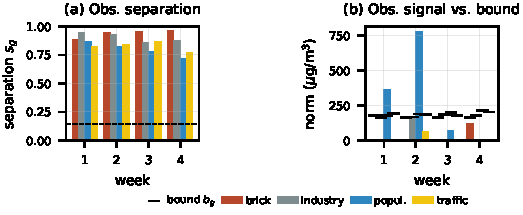
\includegraphics[width=\columnwidth]{figures/fig_observed.pdf}
\caption{Observed New Delhi, weeks 1--4.  \textbf{(a)}~Separation \(s_g\) of each source
group, with the dashed line at \(\tau_\theta=0.141\).  \textbf{(b)}~Norm of each fitted group signal
over the week's readings (bars) and its error bound \(b_g\) of
Theorem~\ref{thm:group_error}(c) at \(\sigma_e=30.68\), \(\delta=0.05\) (ticks).}
\label{fig:observed}
\end{figure}

\noindent\textbf{Group signals against the noise level.}
Theorem~\ref{thm:group_error}(c) with \(\sigma_e=30.68\), \(\operatorname{rank}(\At)=7\)
and \(\delta=0.05\) bounds the error of each group's fitted signal by
\(b_g=156.2/s_g\), which is \(162\)--\(217\,\mu\mathrm g/\mathrm m^3\) for the four groups
(Figure~\ref{fig:observed}(b)).  For the largest group, \(b_g\) is \(0.49\) and \(0.24\)
times its fitted norm in weeks 1 and 2 (population, with norms \(365\) and \(776\)) and
\(2.96\) and \(1.33\) times it in weeks 3 and 4 (population with norm \(67.5\) and brick
kilns with norm \(121.5\)).  At this noise level the bound therefore establishes that the largest group's signal is
resolved in weeks 1 and 2, and does not establish it in weeks 3 and 4.  The bootstrap gives the same split
(Table~\ref{tab:observed_shares}): the 95\% interval of the largest share has width
\(0.25\) and \(0.14\) in weeks 1 and 2, and \(0.94\) and \(0.67\) in weeks 3 and 4.  For AR(1) errors with coefficient \(0.857\), independent across sensors,
\(\|\Sigma\|_2\le(1+0.857)/(1-0.857)\,\sigma_e^2=13.0\,\sigma_e^2\), a level of \(110.7\),
at which the bound exceeds the largest group's norm in every week except week 2.

\noindent\textbf{What the fit explains.}
The projected residual has root mean square \(46\)--\(91\,\mu\mathrm g/\mathrm m^3\) per
reading, against \(1.05\)--\(13.24\) for the total fitted signal (\(2.3\)--\(14.5\%\) of the
residual in each week).  The adequacy test reports no verdict because no calibrated noise model exists.  The bounds above hold under
Assumptions~\ref{ass:model} and~\ref{ass:noise}, and a residual root mean square
\(1.5\)--\(3.0\) times \(\sigma_e\) means that the declared model, the noise level, or both
do not describe these weeks fully.  The shares are fractions of the fitted projected
concentration signal, so they are not emission shares, and because the nuisance terms
are removed first they are not shares of PM\(_{2.5}\) mass.
